\clearpage
\section{Экспериментальная установка -- детектор
\uppercase{LHC}\lowercase{b}}
\label{sec:detector}

Большой адронный коллайдер -- самый большой ускоритель в истории физики 
частиц. Он представляет собой синхротрон, расположенный под землей на 
границе Франции и Швейцарии вблизи Женевы на средней глубине 
приблизительно 100~метров. Поскольку сталкиваемые частицы не являются 
парой частица-античастица, коллайдер состоит из двух отдельных колец, 
имеющих несколько точек пересечения, где и происходят соударения. Длина 
каждого из колец составляет 26.7~километров, а ускоряться в них могут 
протоны и тяжелые ионы. На Большом адронном коллайдере расположены 
четыре основных эксперимента: два эксперимента общего назначения, ATLAS 
и CMS, LHCb, изначально нацеленный на физику тяжелых адронов, и ALICE, 
специализирующийся на физике тяжелых ионов.

Периоды работы БАК, включая тесты и настройку системы БАК, набор 
технических данных и набор данных, предназначенных для физического 
анализа, объединяют и обозначают как Run. В промежутках между ними 
происходит обслуживание и модернизация как ускорителя, так и детекторов. 
Первое улучшение было нацелено, в частности, на увеличение энергии 
столкновения протонов. Run 1 для протонных пучков длился с 2011 до 2012 
года, в течение которых энергия в системе центра масс составляла 
7~и~8~ТэВ. Run 2 длился с 2015 до 2018 года, а энергия соударения 
составляла 13~ТэВ. Run 3 начался в апреле текущего 2022 года, то есть на 
год позже графика.

Эксперимент Large Hadron Collider beauty (LHCb) -- один из четырех 
основных экспериментов, расположенных на Большом адронном коллайдере. 
Изначально LHCb создавался для проведения рекордно точных измерений 
в прелестном и очарованном секторах Стандартной модели, включая 
нарушение $CP$-четности и исследование очень редких распадов. Такие 
опыты предоставляют способ проведения косвенных, но довольно 
чувствительных, проверок с целью обнаружения новой физики вне 
Стандартной модели. Однако с тех пор программа физики на LHCb 
существенно расширилась, и коллаборация привнесла выдающийся вклад 
в обогащение современных знаний об адронной спектроскопии, физике 
тяжелых ионов, экзотических частицах, физике странных частиц и так 
далее. Многим достижениям коллаборации способствуют тщательно 
продуманная архитектура детектора LHCb и многостадийные системы 
обработки данных, которые позволяют реконструировать распады прелестных 
и очарованных частиц эффективно и с высокой точностью.

\begin{figure}%LHCb detector{{{
  \centering
  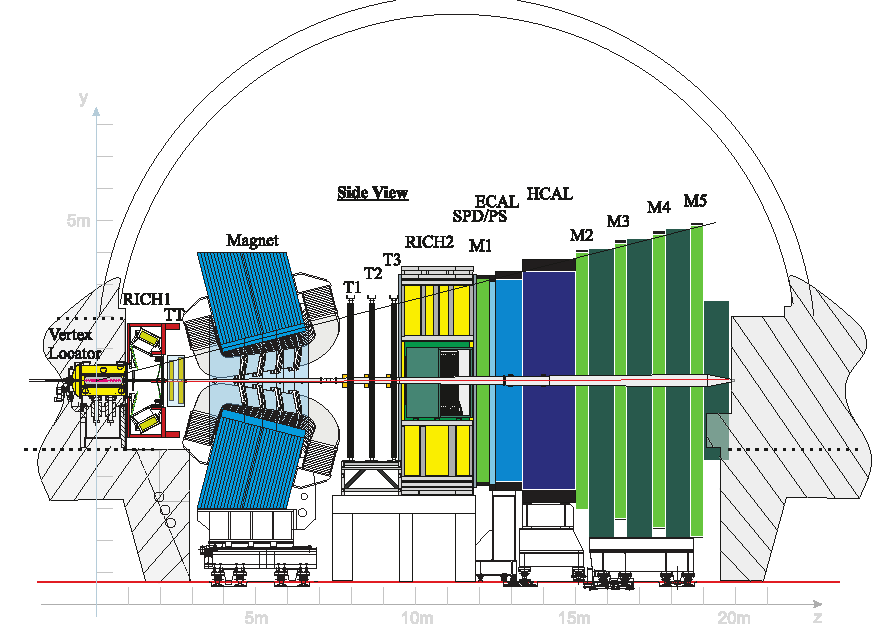
\includegraphics[width=.7\linewidth]{figures/lhcb-detector}
  \caption{Общий вид и основные элементы детектора LHCb.}
  \label{fig:lhcb}
\end{figure}%}}}

Детектор LHCb оптимизирован для сбора и реконструкции прелестных 
и очарованных частиц~\cite{LHCb1, LHCb2}. В протонных соударениях при 
энергии порядка ТэВ рождение $b\bar{b}$ пар происходит существенно чаще 
вдоль линии пучка, поэтому детектор LHCb устроен в виде  одноплечевого 
спектрометра и покрывает угловые интервалы от 0.01 до 3 радиан по 
горизонтали и от 0.01 до 2.5 радиан по вертикали. При таких размерах 
примерно четверть образованных $b\bar{b}$ пар регистрируется детектором. 
Общий вид детектора представлен на рисунке~\ref{fig:lhcb}. Изучение 
прелестных и очарованных барионов в протонных соударениях на БАК требует 
высокоэффективной сепарации сигнала и колоссального количества фона, 
проистекающего из мягких процессов квантовой хромодинамики. Также 
требование высокоточной реконструкции сигнальных процессов позволяет 
достигать хорошего разрешения по массам, времени жизни, угловым 
переменным и прочему. Детекторые системы, составляющие комплекс 
LHCb, оптимизированы для определенных задач.


Трековая система позволяет восстанавливать траектории заряженных частиц, 
а также вершины взаимодействий и распадов. Ее пространственное 
разрешение достаточно велико для идентификации ненулевого расстояния, 
преодолеваемого нерезонансными прелестными и очарованными адронами до их 
распада, что необходимо для снижения фона, обусловленного треками 
частиц, рожденных непосредственно в вершине соударения протонов. Кроме 
того, вкупе с дипольным магнитом, трековая система также позволяет 
с достаточной точностью оценивать импульсы частиц, вследствие чего LHCb 
имеет хорошее разрешение по кинематическим переменным, используемым 
в разнообразных физических анализах.
%
Трековая система состоит из вершинного детектора (VELO), трековых 
станций TT и T1--T3 и дипольного магнита.
%
Вершинный детектор расположен в непосредственной близости от точки 
соударения пучков и представляет собой кремниевый микростриповый 
детектор. Он состоит из сенсоров двух типов, одни из которых 
регистрируют радиальное положение частицы по отношению к линии пучка, 
а другие -- азимутальный угол. Выбор полярных координат позволяет 
ускорить принятие решений триггерной системой. Типичное значение 
эффективности регистрации частиц вершинным детектором составляет 98\%, 
а пространственное разрешение имеет величину около 7~мкм.
%
Из трековых станций, TT расположен перед магнитом и регистрирует все три 
координаты заряженной частицы с эффективностью более 99\% и разрешением 
50~мкм. Остальные три станции расположены после магнита и каждая из них 
состоит из двух частей: внутренней, расположенной ближе к линии пучка, 
и внешней, покрывающей остальную часть телесного угла LHCb. Внутренняя 
часть, как и TT, вновь является кремниевым микростриповым детектором 
и имеет характеристики, подобные TT. Внешняя часть, в свою очередь, 
является дрейфовой камерой, содержащей смесь аргона, CO$_2$ и O$_2$. Ее 
эффективность может превышать 99\%, а разрешение можно грубо оценить 
величиной 200~мкм.
%
В данном анализе использовались только треки, имеющие следы во всех 
частях трековой системы, поскольку они предоставляют наиболее полную 
информацию о частицах.


Протонные пучки для детектора LHCb слегка расфокусируют для достижения 
более стабильной светимости и снижения нагрузки на детектор. Количество 
заряженных частиц, образуемых в соударениях на LHCb, достигает примерно 
100. Разделение частиц разных типов в детекторе позволяет существенно 
сократить фон случайных комбинаций при реконструкции эксклюзивных 
прелестных и очарованных распадов и тоже является требованием 
к детектору LHCb.
%
Система идентификации частиц опирается на информацию из черенковских 
детекторов (RICH1 и RICH2), калориметров (ECAL и HCAL) и мюонных камер 
(M1--M5). Черенковские детекторы основаны на явлении излучения 
Вавилова-Черенкова, которое проявляется, когда скорость заряженной 
частицы в среде оказывается выше скорости света. В такой ситуации 
возникает излучение в конусе с углом $\theta_C = \mathrm{arccos}(c_m/v)$,
где $c_m$ -- скорость света в среде, а $v$ -- скорость заряженной 
частицы. Измерение угла излучения позволяет определить скорость частицы, 
а трековая система, описанная ранее, измеряет импульс. Сравнение этих 
независимых измерений и позволяет определить тип частицы. Черенковские 
детекторы являются основой системы идентификации частиц. Среди четырех 
основных экспериментов на БАК только LHCb оснащен черенковскими 
детекторами, что делает его уникальным и открывает дорогу для более 
тонкого изучения распадов тяжелых адронов. Наличие двух черенковских 
детекторов продиктовано тем фактом, что угол $\theta_C$ при больших 
импульсах выходит на насыщение и перестает предоставлять достаточно 
точную информацию о типе частицы. Для учета этого эффекта один из 
детекторов содержит аэрогель и газ C$_4$F$_{10}$, а другой -- только газ 
CF$_4$. Таким образом, они оказываются чувствительны к типам частиц 
в разных интервалах импульса и дополняют друг друга.
%
Калориметры служат в основном для измерения энергий частиц, включая 
электрически нейтральные. Как электромагнитный, так и адронный 
калориметры имеют меньшие размеры ячеек вблизи линии пучка для 
компенсации разницы в множественности частиц. Электромагнитный 
калориметр имеет чередующуюся структуру из сцинтилляторов и свинца. 
Толщина калориметра составляет 25 радиационных длин, так что 
электромагнитные ливни от фотонов и электронов оказываются полностью 
поглощенными. Адронный калориметр (HCAL) состоит из чередующихся плиток 
сцинтиллятора и железа. Ввиду пространственных ограничений, толщина этой 
части калориметра ограничена 5.6 длинами взаимодействия, и поэтому он не 
успевает поглотить ливень частиц целиком, а лишь предоставляет оценку 
энергий адронов. Основной задачей HCAL является быстрое измерение 
энергии для последующего использования триггерной системой.
%
Мюонные камеры расположены дальше всех от точки соударения протонов 
и предоставляют необходимые данные как для идентификации мюонов, так 
и для отбора событий. Оба этих критерия являются неотъемлемой частью 
многих исследований на LHCb. Одна из мюонных камер, М1, расположена 
перед калориметром, что способствует измерению поперечного импульса, 
используемого системой отбора событий. М1 представляет собой газовый 
электронный умножитель, а остальные детекторы М2--М5 -- 
многопр\'{о}водные пропорциональные счетчики. Между каждой камерой 
М2--М5 расположен слой железа, действующий в качестве аппаратного 
фильтра высокоэнергичных мюонов. Детекторы М1--М3 позволяют с высокой 
скоростью оценить поперечный импульс мюона отдельно от трековой системы. 
Относительная точность такой оценки составляет 20\%.


Задачей системы триггеров является эффективная реконструкция и отбор 
интересующих событий непосредственно во время сбора данных. Она 
контролирует частоту событий и количество информации так, чтобы нагрузка 
оставалась в пределах производительности доступной долгосрочной памяти.
%
Триггер LHCb состоит из двух частей: аппаратной 
и программной~\cite{LHCb-trigger-Run1, LHCb-trigger-Run2}. Решения 
аппаратной части основаны на информации из калориметров и мюонных камер, 
а события отбираются по большим поперечным импульсам и энергиям 
продуктов распадов прелестных и очарованных адронов. Большая величина 
поперечного импульса, измеренного мюонными камерами М1--М3 без 
использования данных трековой системы, гарантирует прохождение 
аппаратного этапа отбора. Кроме того, аппаратный триггер устанавливает 
верхний предел на множественность заряженных частиц, поскольку события 
с большой множественностью реконструируются со значительными 
погрешностями. Аппаратный отбор сокращает частоту событий с 40~МГц до 
1~МГц, на которой может работать упрощенный алгоритм реконструкции 
событий, а вместе с ним и программный триггер.
%
Программный отбор производится в две стадии. На первой восстанавливаются 
треки событий, а также на основе данных вершинного детектора 
устанавливается точка соударения протонов, что позволяет находить 
отклонения треков от нее. Треки, имеющие следы во всех частях трековой 
системы и существенно отклоненные от исходной вершины свидетельствуют 
о произошедшем распаде $b$ или $c$ кварка. Кроме того, отбираются 
события с большой инвариантной массой двух мюонов. На второй стадии 
частично восстанавливаются распады частиц и производится более глубокий 
анализ актуальности события.
%
Событие может пройти отбор как благодаря частицам распада, 
непосредственно изучаемого в анализе, так и благодаря частицам 
какого-либо стороннего распада. Этот факт отражен в данных наличием 
переменной, содержащей информацию о том, по какой именно причине данное 
событие прошло отбор во время сбора данных. Эта переменная может 
принимать два значения: триггер сработал на сигнал (TOS) или триггер 
сработал независимо от сигнала (TIS).
